\documentclass[a4paper]{article}
\usepackage[UTF8]{ctex}
\usepackage{geometry}
\usepackage{graphicx}
\usepackage{url}
\usepackage{multirow}
\usepackage{array}
\usepackage{booktabs}
\usepackage{url}
\usepackage{enumitem}
\usepackage{graphicx}
\usepackage{float}
\usepackage{amssymb}
\usepackage{amsmath}
\usepackage{subfig}
\usepackage{longtable}
\usepackage{pifont}
\usepackage{color}
\usepackage{listings}
\usepackage{xcolor}

\allowdisplaybreaks

\geometry{a4paper, scale=0.78}

% \begin{figure}[H]
%     \centering
%     \includegraphics[width=.55\textwidth]{E.png}
%     \caption{矩阵与列向量的乘法}
%     \label{fig:my_label_1}
% \end{figure}

% \left\{
% \begin{array}{ll}
%       x+2x+z=2 & \\
%       3x+8y+z=12 & \\
%       4y+z=2
% \end{array}
% \right.

% \begin{enumerate}[itemindent = 1em, itemsep = 0.4pt, parsep=0.5pt, topsep = 0.5pt]

% \end{enumerate}

%\stackrel{a}{\longrightarrow}

\title{Probability Graph 05 Markov Network}
\author{Chen Gong}
\date{27 November 2019}

\begin{document}
\maketitle
上一小节中,我们分析了有向图Bayesian Network,得到了因子分解法,$p(x) = \prod_{i=1}^N p(x_i|x_{pa(i)})$。虽然,有向图中可以方便直观的表达条件独立性,但是它也有它的局限性。也就是我们提到的对于Head to Head的结构来说,当中间节点被观察到的时候,反而是两端的节点是相关的。这违反了条件独立性的特点,也就是当某些变量被观察到时,其他变量之间是独立的特点,这种情况有点反常,并不太好办。

但是,在无向图中就完全不会出现这样的情况,因为本来就没有方向,而且在无向图中也有类似的D-Separation性质。
\section{Condition Independence in Markov Network}
Markov中的条件独立,大致可以被我们分成三种情况,Global Markov,Local Markov和Pair Markov。
\subsection{Global Markov}
假设现在有三个集合$X_A \bot X_B | X_C$,我们想得到$a\in X_A,b\in X_B$之间相互独立,这个应该怎么办?我们给出,只有$a$和$b$的中间节点至少有一个位于$c$中,那么我们就可以得到$a \bot c$。

\subsection{Local Markov}
我们以下图的一个Markov Network为例,
\begin{figure}[H]
    \centering
    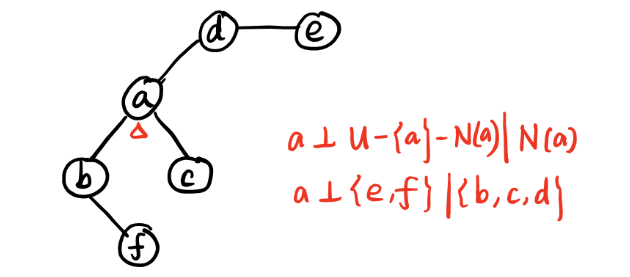
\includegraphics[width=.55\textwidth]{微信图片_20191126225153.png}
    \caption{Markov Network示意图}
    \label{fig:my_label_1}
\end{figure}

用文字的语言来描述就为$a\bot\{$全集$-a-$邻居$\}|$邻居。那么在这个图中,我们就可以表示为$a\bot\{e,f\}|\{b,c,d\}$。

\subsection{Pair Markov}
成对马尔可夫性质可以被我们描述为:$x_i\bot x_j|x_{-i-j}\ (i\neq j)$。其中,$x_{-i-j}$为从全集中去掉$x_i$和$x_j$而留下了的集合。

那么条件独立性就可以提现在,Global,Local和Pair中。其中Global$\Leftrightarrow$Local$\Leftrightarrow$Pair。也就是这三种条件独立的方法得到的结果是一样的。

\section{因子分解法}
我们想一想在一个无向图中,如何来体现我们想要的条件独立性。这里的引入和之前的不太一样,我们首先需要引入几个概念。\textbf{团}:这是一个关于节点的集合,集合中的节点是相互连通的。而最大团,就很好理解了吧,也就是最大的连通子集。我们可以将无向图的分离定义到团上,我们假设$c_1,c_2,\cdots,c_k$表示为团。那么,我们可以将联合概率定义为:
\begin{equation}
    p(x) = \frac{1}{Z}\prod_{i=1}^k \phi_{i} (x_{c_i})
\end{equation}

其中,$z$是归一化因子,因为没有归一化因子的话,这不能被称为一个概率分布,因为概率分布首先就要保证和等于1。那么,$z$被定义为
\begin{equation}
    z = \sum_x \prod_{i=1}^k\phi_i(x_{c_i}) = \sum_{x_1}\cdots\sum_{x_N} \prod_{i=1}^k\phi_i(x_{c_i})
\end{equation}

\section{Gibbs Distribution和Exponential Distribution}
这个部分是上面部分的一个加深理解,首先我们需要总结一下。

1. Global Markov:$X_A \bot X_C | X_B$。也就是$X_A$和$X_B$之间所有的连接都必须在$X_C$中,此时在无向图中满足全局马尔可夫性。

2. Local Markov Network:$x_i\bot x_{-i-nb(i)}|x_{nb(i)}$,其实nb(i):neighbor of node i。

3. Pair Markov:$x_i \bot x_j|x_{-i-j}$。

1$\Leftrightarrow$2$\Leftrightarrow$3$\Leftrightarrow$因子分解(基于最大团)。这里面实际上是有个Hammesley-Clifford定理的,这个定理的证明非常的困难,我们这里就不做过多的阐述(实际上我也看的有点懵逼,有需求的小伙伴可以查下Hammesley-Clifford定理的证明)。

\noindent 因子分解:

在我们之前的定义中,
\begin{equation}
    p(x) = \frac{1}{Z}\prod_{i=1}^k \phi_i(x_{c_i})
\end{equation}

$c_i$:最大团;$x_{c_i}$:最大团的随机变量集合;$\phi(x_{c_i})$:势函数,必须为正。这里的概念都是来自于统计物理学和热力学的过程。这里的势函数还有可以做文章的地方。

因为,势函数必定为正,我们可以将势函数表达为$\phi(x_{c_i}) = \exp\{ -E(x_{c_i}) \}$。其中,$E(x_{c_i})$称为Energy function。实际上用这种形式表达的$p(x)$,为Gibbs Distribution,或者又被称之为Boltzman Distribution。有了$\phi(x_{c_i})$的形式,我们可以进一步推导得:
\begin{equation}
    p(x) = \frac{1}{Z}\prod_{i=1}^K\phi(x_{c_i}) = \frac{1}{Z}\prod_{i=1}^K \exp\{ -E(x_{c_i}) \} = \frac{1}{Z}\exp\{ - \sum_{i=1}^k E(x_{c_i}) \}
\end{equation}

我们再来回顾一下指数族分布,指数族分布的通用表达形式为:
\begin{equation}
    p(x) = h(x)\exp\{ \eta^T\phi(x) - A(\eta) \} = h(x)\frac{1}{Z(\eta)}\exp\{ \eta^T\phi(x)\}
\end{equation}

在这里我们把$\exp\{ - A(\eta) \}$,直接记为$Z(\eta)$。大家观察就会发现势函数也就是Gibbs Distribution就是一个指数族分布。Gibbs是来自统计物理学,形式上和指数族分布时一样的。而指数族分布实际上是由最大熵分布得到的,那么我们可以理解Gibbs分布也是有最大熵原理得到的。而马尔可夫随机场(Markov Random Field)实际上等价于Gibbs分布。至于为什么?这实际上全部都在Hammesley-Clifford定理中,有兴趣的同学,请自行查阅。















\end{document}